\chapter{Experiments}
\noindent In this chapter, we compare the performance of the PDKind engine with two Golem engines, SPACER and KIND.

\section{Methodology}
\noindent We measured the performance of each engine on the benchmarks from the CHC-COMP\footnote{\url{https://github.com/orgs/chc-comp/repositories}} in the year 2021. CHC-COMP is an annual competition that compares the performance of multiple CHC solvers.

We ran all three engines on all benchmarks from the LRA-TS category of CHC-COMP. This category focuses on transition systems over linear real arithmetic, with 498 benchmarks in it. In these experiments, the goal is to 1) verify the correctness of the PDKind engine by comparing results with the other two engines, and 2) find out how PDKind performs in comparison with the other two engines, where Spacer is the default engine for Golem, and KIND is the best-performing engine for LRA-TS in Golem.

\section{Results}
\noindent All experiments were conducted on a machine with an AMD EPYC 7452 32-core processor and 8 × 32 GiB of memory; the timeout was set to 300 s, where for each engine 8 processes were running in parallel. During the experiments, there were no conflicts in answers between the engines. We can consider this fact as strong proof of the correctness of our engine.

In the table \ref{tab:results}, we can see that PDKind is significantly better than Spacer in the number of SAT results and matched it in the number of UNSAT results. KIND, however, outperformed both engines in both SAT and UNSAT results.

\renewcommand{\figurename}{Table}
\begin{figure}[H]
\centering
\begin{tabular}{|c|c|c|c|}
\hline
Result & PDKind & Spacer & KIND \\
\hline
SAT & 242 & 214 & 260 \\
\hline
UNSAT & 68 & 70 & 84 \\
\hline
TIMEOUT & 188 & 214 & 154 \\
\hline
\end{tabular}
\caption{Number of solved benchmarks from LRA-TS category} % Adds the caption
\label{tab:results}
\end{figure}

In Figure \ref{fig:sat_indet_comparison} (The scale on both axes is logarithmical and represents the evaluation time in seconds), we compare the SAT results of the engines. In the first plot, we compare PDKind with Spacer. We can see that in most cases, PDKind is at least slightly faster than Spacer. In the second plot, where we compare PDKind with KIND, it is obvious that KIND outperforms our engine, but we can observe several cases where PDKind solved the problem in the given timespan of 300 seconds, but KIND timed out.

In Figure \ref{fig:unsat_indet_comparison}, we compare the UNSAT results of the engines. In both cases, our engine doesn't perform as well as the other engine, but in the first case, the performance of the PDKind engine is at least comparable with the Spacer engine, where the times are mostly similar, in some cases better for Spacer, in other better for PDKind.

\renewcommand{\figurename}{Figure}
\begin{figure}[h!]
    \centering
    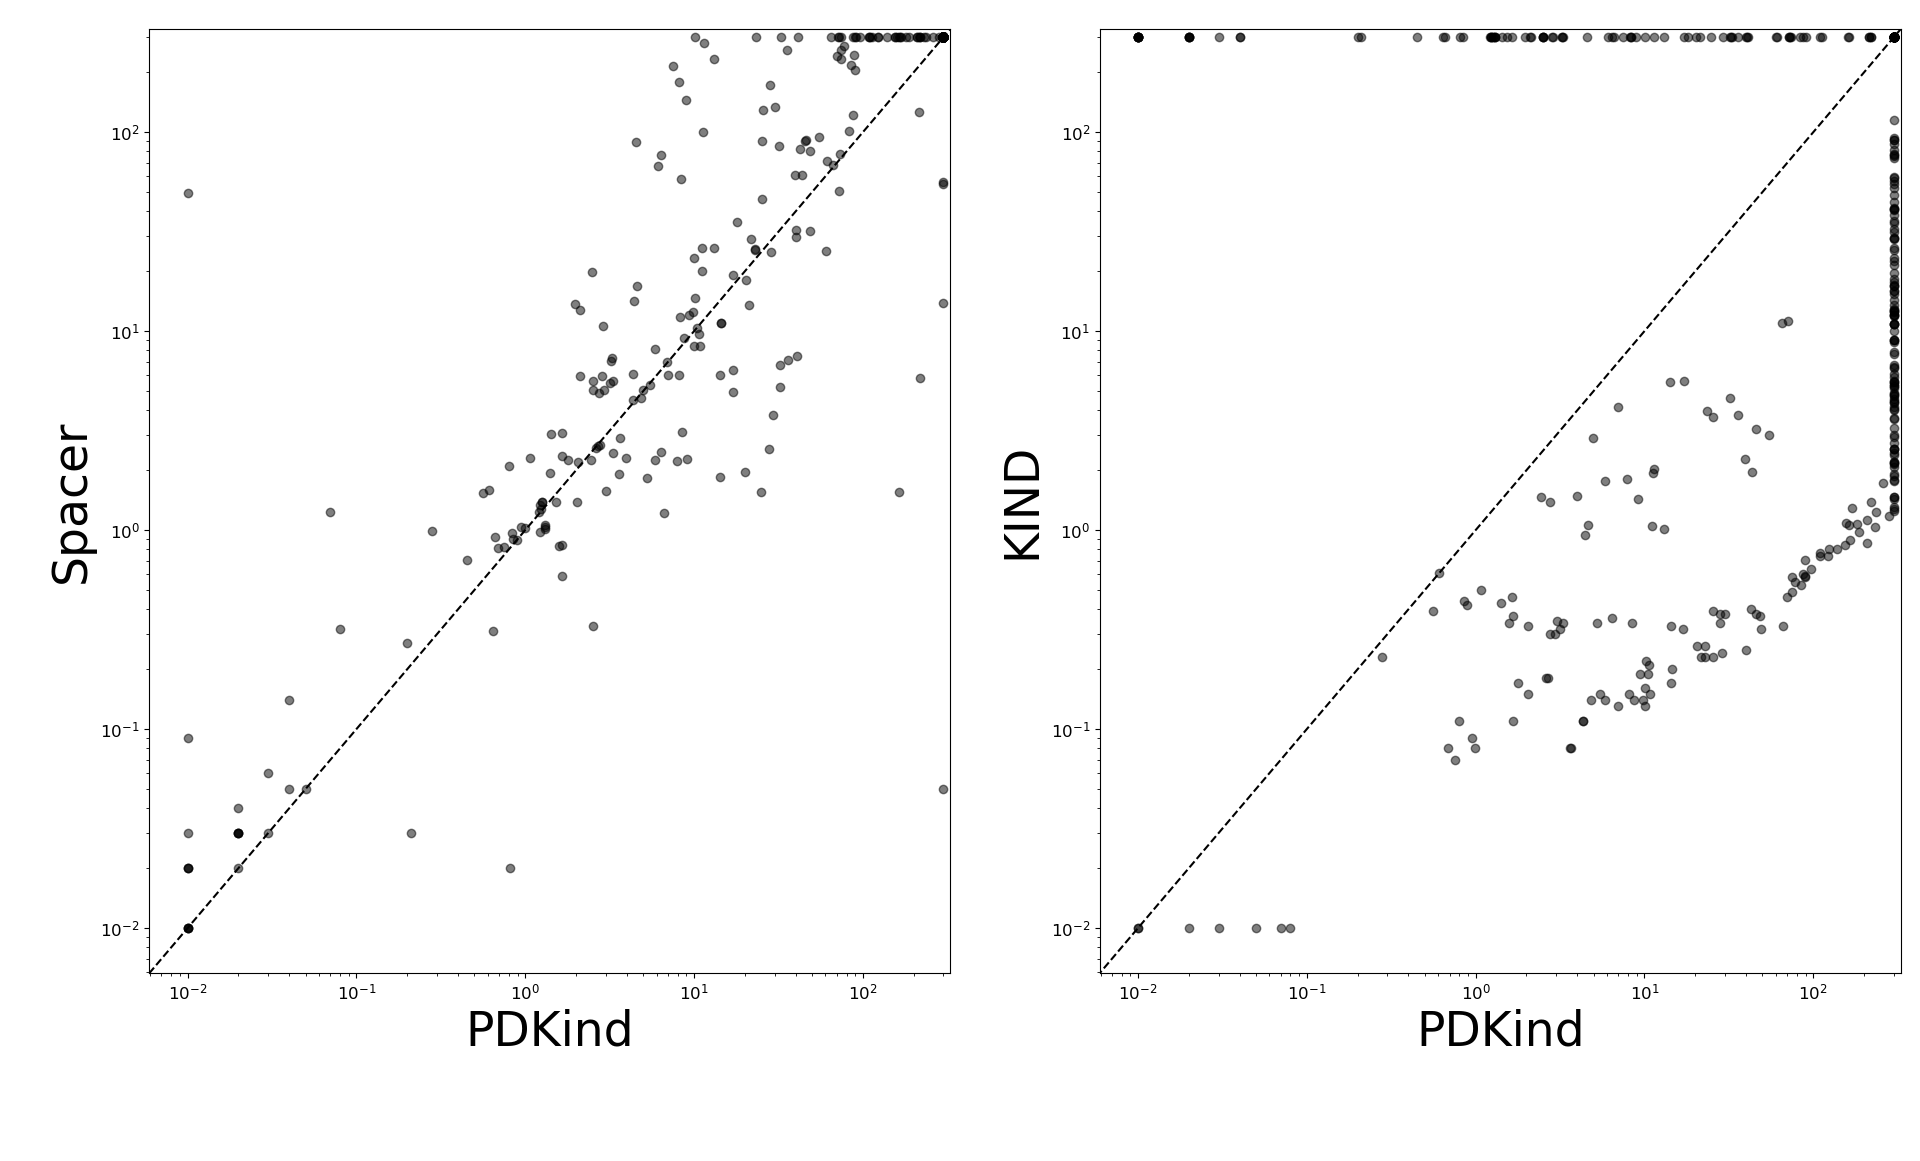
\includegraphics[width=\textwidth]{img/golem_sat_scatter.png}
    \caption{Time Comparison: SAT results}
    \label{fig:sat_indet_comparison}
\end{figure}

\begin{figure}[h!]
    \centering
    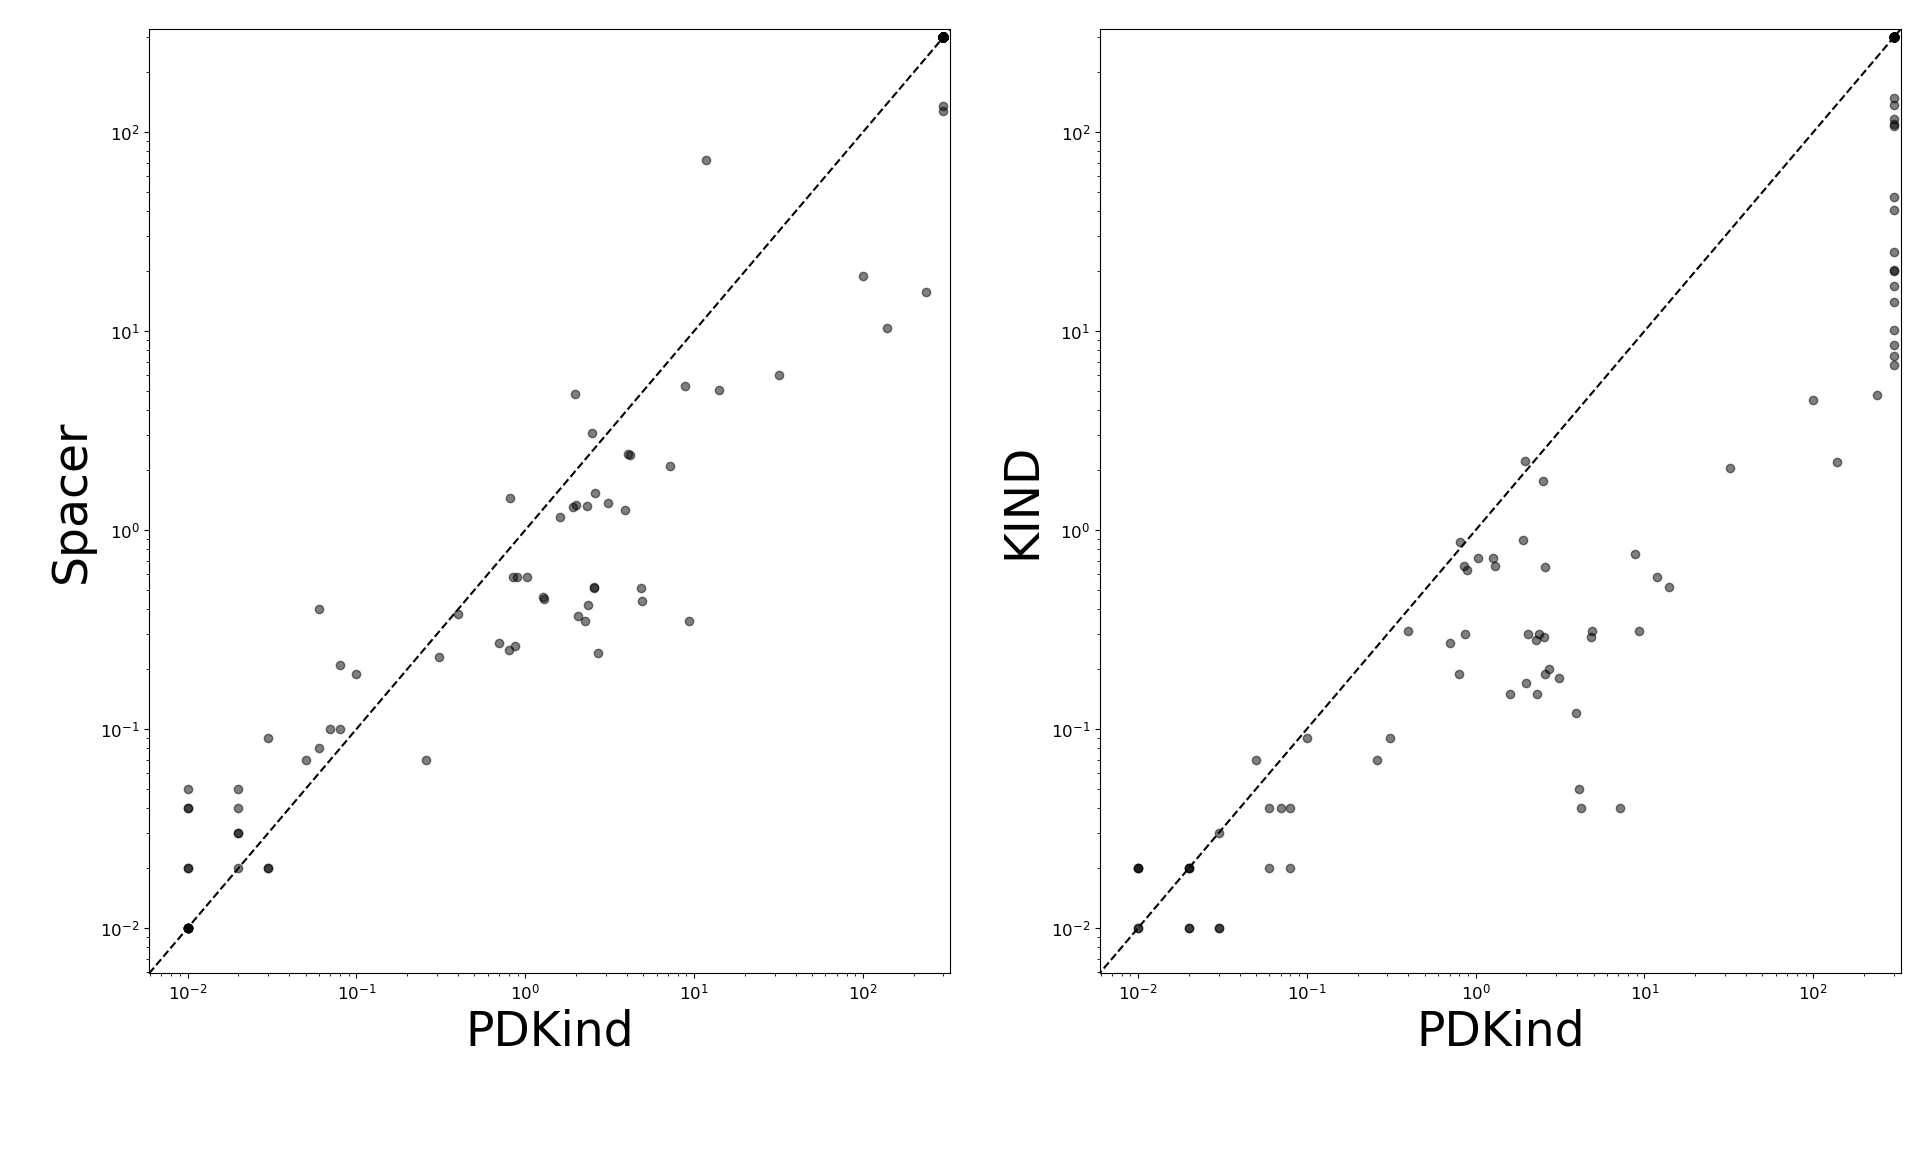
\includegraphics[width=\textwidth]{img/golem_unsat_scatter.png}
    \caption{Time Comparison: UNSAT results}
    \label{fig:unsat_indet_comparison}
\end{figure}
